%FRAGEN:
%U_0 (IM AP 2.28)??
%GAIN IN RECHNUNGEN??
%
%
%
%
%
%
\subsection[]{Verifikation der Funktion eines phasenempfindlichen Gleichrichters}
Mit dem linken Ausgang des Funktionsgenerators (ohne die Beschriftung \enquote{phase shift}) lassen sich die Spannungsamplituden variieren.
Es wird eine konstante Spannung gewählt.
%𝑈0 = 2,28 V nach Altprotokoll(?)
%5.1 so semi erfüllt(?)
%
Im nächsten Schritt wird der Schaltplan \textbf{SCHALTPLAN REFERENZIEREN} aufgebaut,
um die Funktionsweise eines phasenempfindlichen Gleichrichters zu verifizieren.
Dies findet ohne Verwendung des Tiefpasses statt.
Der Gain Regulierer des Verstärkers hat einen Wert von 1 und der Gain Regulierer des Lock-in Detektors einen Wert von 20.
%% FRAGE: MUSS MAN DAS IN DER RECHNUNG BERÜCKSICHTIGEN?
Mit dem Phasenschieber werden insgesamt fünf verschiedene Phasenverschiebungen $\phi$ eingestellt,
die in Abbildung \ref{fig:phasenunterschiede} einzusehen sind.
%
\begin{figure}%
    \begin{subfigure}{0.5\textwidth}%
    \centering%
    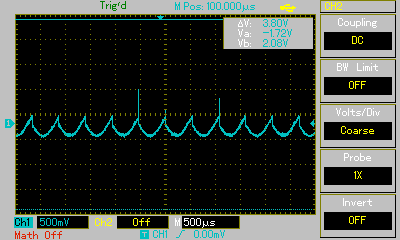
\includegraphics[width = 7.3cm]{./Oszilloskop Bilder/png/5.2/1 MAP002.png}%
    \caption{$\phi = \qty[]{0}{\degree}$}%
    \label{fig:phase1}%
    \end{subfigure}%
    %
    \hfill% Fills available space in the center -> space between figures
    \begin{subfigure}{0.5\textwidth}%
    \centering%
    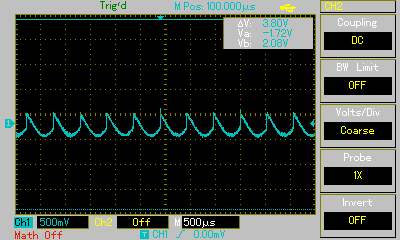
\includegraphics[width = 7.3cm]{./Oszilloskop Bilder/png/5.2/2 MAP003.png}%
    \caption{$\phi = \qty[]{45}{\degree}$}%
    \label{fig:phase2}%
    \end{subfigure}%
    %
    \hfill
    \begin{subfigure}{0.5\textwidth}%
    \centering%
    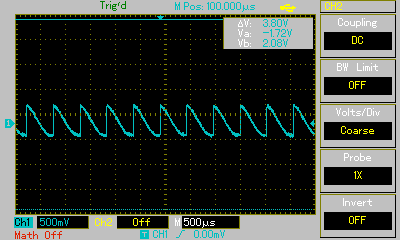
\includegraphics[width = 7.3cm]{./Oszilloskop Bilder/png/5.2/3 MAP004.png}%
    \caption{$\phi = \qty[]{90}{\degree}$}%
    \label{fig:phase3}%
    \end{subfigure}%
    %
    \hfill% Fills available space in the center -> space between figures
    \begin{subfigure}{0.5\textwidth}%
    \centering%
    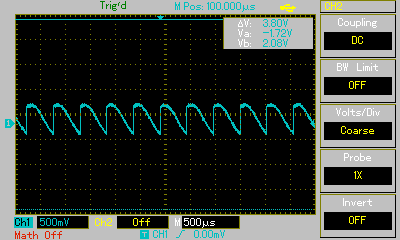
\includegraphics[width = 7.3cm]{./Oszilloskop Bilder/png/5.2/4 MAP005.png}%
    \caption{$\phi = \qty[]{135}{\degree}$}%
    \label{fig:phase4}%
    \end{subfigure}%
    %
    \hfill
    \begin{subfigure}{0.5\textwidth}%
    \centering%
    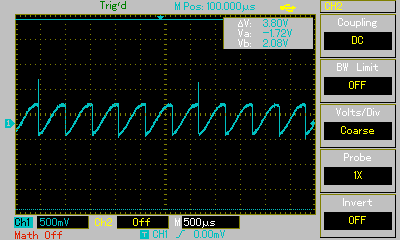
\includegraphics[width = 7.3cm]{./Oszilloskop Bilder/png/5.2/5 MAP006.png}%
    \caption{$\phi = \qty[]{180}{\degree}$}%
    \label{fig:phase5}%
    \end{subfigure}%
    %
    \caption{Spannungsverläufe für unterschiedliche Phasen}%
    \label{fig:phasenunterschiede}%
\end{figure}%
%  
%Anhand der Abbildung \ref{fig:phasenunterschiede}
%

\noindent
Schaltet man den Tiefpass hinzu, ergeben sich je nach Phase $\phi$ die Spannungsamplituden $U$ in Tabelle \ref{tab:u_out_tp_ohne_noise}.
%Spannungsamplitude von channel 1:
% 871.2
% 712.8
% 653.4
% 613.8
% 455.4
% 950.4
% 1190  
% 990.0
% 1170  
% 1030  
\begin{table}
    \centering
    \caption[]{Amplitude der Ausgangsspannung nach Integration durch den Tiefpass}
    \label{tab:u_out_tp_ohne_noise}
    \sisetup{table-format=3.0}
    \begin{tabular}[]{S c S[table-format=2.2]}
        \toprule
        {$\phi / \unit[]{\degree}$} & {$\phi / \unit[]{\radian}$} & {$U / \unit[]{\volt}$} \\
        \midrule
           0 &     0          & -0.10 \\
          45 & $    \pi / 4 $ & -0.10 \\
          90 & $    \pi / 2 $ &  0.04 \\
         135 & $ 3  \pi / 4 $ &  0.18 \\
         180 & $    \pi     $ &  0.28 \\
         225 & $ 5  \pi / 4 $ &  0.26 \\
         270 & $ 3  \pi / 2 $ &  0.14 \\
         300 & $ 5  \pi / 3 $ &  0.06 \\
         315 & $ 7  \pi / 4 $ &  0.00 \\
         330 & $ 11 \pi / 6 $ & -0.06 \\
        \bottomrule
%-100.0
%-100.0
%  40.0
% 180.0
% 280.0
% 260.0
% 140.0
%  60.0
%   0.0
% -60.0
    \end{tabular} 
\end{table}
%
Da die Spannungswerte gemäß \textbf{REFERENZ!!!!} $2 \pi$-periodisch sein sollen, wird eine Ausgleichsrechnung mit der Funktion 
\begin{align}
    \label{eq:ausgleich_tp_ohne_noise}
    U(\phi) = A \cos{\left(B \phi + C\right)} + D 
\end{align}
durchgeführt, was mittels der Funktion \texttt{curve\_fit} aus dem Python \cite{python} Paket \texttt{scipy.optimize} \cite[]{scipy} realisiert wird.
Es ergibt sich Plot \ref{eq:ausgleich_tp_ohne_noise} mit den Parametern
\begin{align*}
    A &= \left(\num[]{-0.2002} \pm \num[]{0.0055}\right) \, \unit{\volt} & B &=  \num[]{0.9938} \pm \num[]{0.0208} \\
    C &= \num[]{-0.2768} \pm \num[]{0.0779} & D &= \left(\num[]{0.0869} \pm \num[]{0.0054}\right) \, \unit[]{\volt} \\
\end{align*}
% cosinus für av_ch2:
% a = -0.20018493
% b = 0.99376117
% c = -0.27683892
% d = 0.08687120
%fehler:
%[0.00549263 0.02075618 0.07790146 0.0054004 ]
%
\begin{figure}
    \includegraphics*[]{build/B01_ausgleichsplot.pdf}
    \caption[]{Ausgleichsfunktion \eqref{eq:ausgleich_tp_ohne_noise} zu den Werten aus Tabelle \ref{tab:u_out_tp_ohne_noise}}
    \label{fig:ausgleichsplot1}
\end{figure}

\noindent Vergleicht man die Ergebnisse mit \textbf{REFERENZ!!!}, so ergibt sich mit
\begin{align*}
    U_0 = \frac{\pi}{2} A = \left(-0.314 \pm 0.009\right) \, \unit[]{\volt}
\end{align*}
%U_0 =  -0.314+/-0.009